\documentclass[12pt]{article}
\usepackage{amsmath}
\usepackage{graphicx}
\usepackage{hyperref}
\usepackage[utf8]{inputenc}
\usepackage{listings}  % Use listings for code blocks
\usepackage{xcolor}

\lstset{
    basicstyle=\ttfamily\footnotesize,
    keywordstyle=\color{blue},
    stringstyle=\color{red},
    commentstyle=\color{green},
    showstringspaces=false,
    breaklines=true,
    frame=single,
    numbers=left,
    numberstyle=\tiny,
    stepnumber=1,
    numbersep=10pt
}


% Redefine the section command to include a dot after the number
\renewcommand\thesection{\arabic{section}.}
\renewcommand\thesubsection{\thesection\arabic{subsection}.}
\renewcommand\thesubsubsection{\thesubsection\arabic{subsubsection}.}

\title{ME/EE/CS 133a Homework 1}

\author{Baaqer Farhat}

\date{10–07–24}

\begin{document}

\maketitle

\section{Problem 1}

\begin{itemize}

\item (a) 

There exists 5 degrees of freedom. A Rigid Body in 3D space has 6 possible Degrees of Freedom bieng (x, y, z) and (pitch, yaw, roll).
A line segment has no thickness so its incapable of achieving the roll rotational DOF. A line segment is 2 dimensional. 

\item (b)

There exists 5 degrees of freedom. A Rigid Body in 3D space has 6 possible Degrees of Freedom bieng (x, y, z) and (pitch, yaw, roll). A 
torus can move along translational axis (x, y, z) and is limited by 1 (rotating about its center) rotational axis (pitch, yaw, roll). 
\item (c)

6 DOFs. 5 from part (a) and the 6th comes from the length of the segment. The length is an additional property of the line segment that 
can be varied independently, and thus contributes 1 extra degree of freedom to the total number needed to describe the segment in 3D 
space.


\item (d)

7 Dofs. 5 from part (b) similar to part (c) the major and minor axis add 2 additional DOFS.

\end{itemize}

\section{Problem 2}

\begin{itemize}
    \item (a)
    Lets use Gublers formula for calculating the degrees of freedom. Formula states that 

    \begin{center}
        \[
        \text{DOF} = m(N) + \sum_{i=1}^{J} f_i
        \]
        \end{center}
        
        \end{itemize}

        Using the formula:
        \[
        \text{DOF} = 3(N) + \sum_{i=1}^{J} f_i = 3(2) - 2 = 4
        \]
        
        Therefore, the system has 4 degree of freedom.
        \item (b)
        Using the formula:
        \[
        \text{DOF} = 3(N) + \sum_{i=1}^{J} f_i = 3(3) - 2(2) = 5
        \]
        
        Thus, the system has 5 degree of freedom.
\end{itemize}

\section{Problem 3}
The human arm non iclusing wrist consists of 5 Fingers, 4 are identical and thumb is different. The DOFS per joint per finger group 
are as follows:

\subsection*{Thumb:}
- The \text{base of the thumb} moves:
  \begin{itemize}
      \item \textit{Up/down} (1 DOF)
      \item \textit{Forward/backward} (1 DOF)
  \end{itemize}
  
- The \text{knuckle of the thumb} moves:
  \begin{itemize}
      \item \textit{Up/down} (1 DOF)
      \item \textit{Left/right} (1 DOF)
  \end{itemize}
  
- The \text{thumb tip joint} moves:
  \begin{itemize}
      \item \textit{Up/down} (1 DOF)
  \end{itemize}
  Total for the thumb = 5 DOFs.

\subsection*{Fingers (Index, Middle, Ring, Pinky):}
Each finger has the following joints:
\begin{itemize}
    \item \text{Knuckle}:
      \begin{itemize}
        \item \textit{Up/down} (1 DOF)
        \item \textit{Left/right} (1 DOF)
      \end{itemize}
      
    \item \text{Middle joint of the finger}:
      \begin{itemize}
        \item \textit{Up/down} (1 DOF)
      \end{itemize}
      
    \item \text{Fingertip joint}:
      \begin{itemize}
        \item \textit{Up/down} (1 DOF)
      \end{itemize}
\end{itemize}

So, each finger has 4 DOFs, and for 4 fingers:
\[
4 \times 4 = 16 \, \text{DOFs}.
\]

\subsection*{Total Degrees of Freedom:}
The total DOFs for the hand are:
\[
16 \, (\text{DOFs for 4 fingers}) + 5 \, (\text{DOFs for the thumb}) = 21 \, \text{DOFs}.
\]


\section{Problem 4}

\begin{itemize}
    \item (a)
    
    Given that the hips and pelvis are fixed, the legs and ankles can move freely. The degrees of freedom are:

    \begin{itemize}
        \item \textbf{Ankles}: 1 DOF per leg (up/down movement).
        \item \textbf{Knees}: 1 DOF per knee (up/down movement).
        \item \textbf{Hip}: 1 rotational DOF for pedaling motion.
    \end{itemize}
    
    Total DOFs:
    \[
    \text{Total DOFs} = 2 \, \text{(ankles)} + 2 \, \text{(knees)} + 1 \, \text{(hip)} = 5 \, \text{DOFs}.
    \]
    

    \item (b)
    
    When standing on the pedals, the hips and pelvis are not fixed. The degrees of freedom are:

    \begin{itemize}
        \item \textbf{Ankles}: 1 DOF per leg (up/down movement).
        \item \textbf{Knees}: 1 DOF per knee (up/down movement).
        \item \textbf{Hips}: 3 DOFs per leg (Forward/backward, left/right, in/out rotation).
    \end{itemize}
    
    Total DOFs:
    \[
    \text{Total DOFs} = 2 \, \text{(ankles)} + 2 \, \text{(knees)} + 6 \, \text{(hips)} = 11 \, \text{DOFs}.
    \]

\end{itemize}



\section{Problem 5}
\subsection*{Geometric Derivations}

We start by using the Pythagorean theorem to solve for the distance \( r \), angle \( \beta \), and angle \( \gamma \). Then, we calculate the angles \( \theta_1, \theta_2, \theta_3, \theta_4 \) as described below.

\subsection*{Pythagorean Theorem for \( r \)}

The distance \( r \) from the origin to point \( B \) is calculated using the Pythagorean theorem:

\[
r = \sqrt{X_B^2 + Y_B^2}
\]

where:

\[
X_B = d + c \cdot \cos(\phi)
\]

and

\[
Y_B = c \cdot \sin(\phi)
\]

This represents the distance from the base pivot to point \( B \) in the four-bar linkage.

\subsection*{Law of Cosines for \( \beta \)}

The angle \( \beta \) is derived using the law of cosines:

\[
\cos(\beta) = \pm\frac{a^2 + r^2 - b^2}{2 \cdot a \cdot r}
\]

Solving for \( \beta \):

\[
\beta = \pm\cos^{-1} \left(\frac{a^2 + r^2 - b^2}{2 \cdot a \cdot r} \right)
\]

\subsection*{Angle \( \gamma \)}

The angle \( \gamma \) can be found using the \( \text{atan2} \) function, which accounts for the correct quadrant:

\[
\gamma = \text{atan2}(Y_B, X_B)
\]

This handles both the angle's direction and ensures the correct quadrant is considered.

\subsection*{Full Expression for \( \theta \)}

The angle \( \theta \) is derived from the combination of \( \gamma \) and \( \beta \), where:

\[
\theta = \text{atan2}(Y_B, X_B) \pm \cos^{-1}\left( \frac{a^2 + \left(X_B^2 + Y_B^2\right) - b^2}{2 \cdot a \cdot \sqrt{X_B^2 + Y_B^2}} \right)
\]

with:

\[
X_B = d + c \cdot \cos(\phi)
\]
\[
Y_B = c \cdot \sin(\phi)
\]

\subsection*{Possibilities for \( \theta \)}

Finally, the angles \( \theta_1 \) and \( \theta_2 \) are calculated as (from original theta):

\[
\theta_1 = \gamma + \beta
\]
\[
\theta_2 = \gamma - \beta
\]

By adding \( 2\pi \) to each, we get \( \theta_3 \) and \( \theta_4 \):

\[
\theta_3 = \theta_1 + 2\pi
\]
\[
\theta_4 = \theta_2 + 2\pi
\]
\subsection*{Configuration Space Plots}

The following figures show the configuration space of the four-bar linkage for different values of \( c \):.


\begin{figure}[h!]
    \centering
    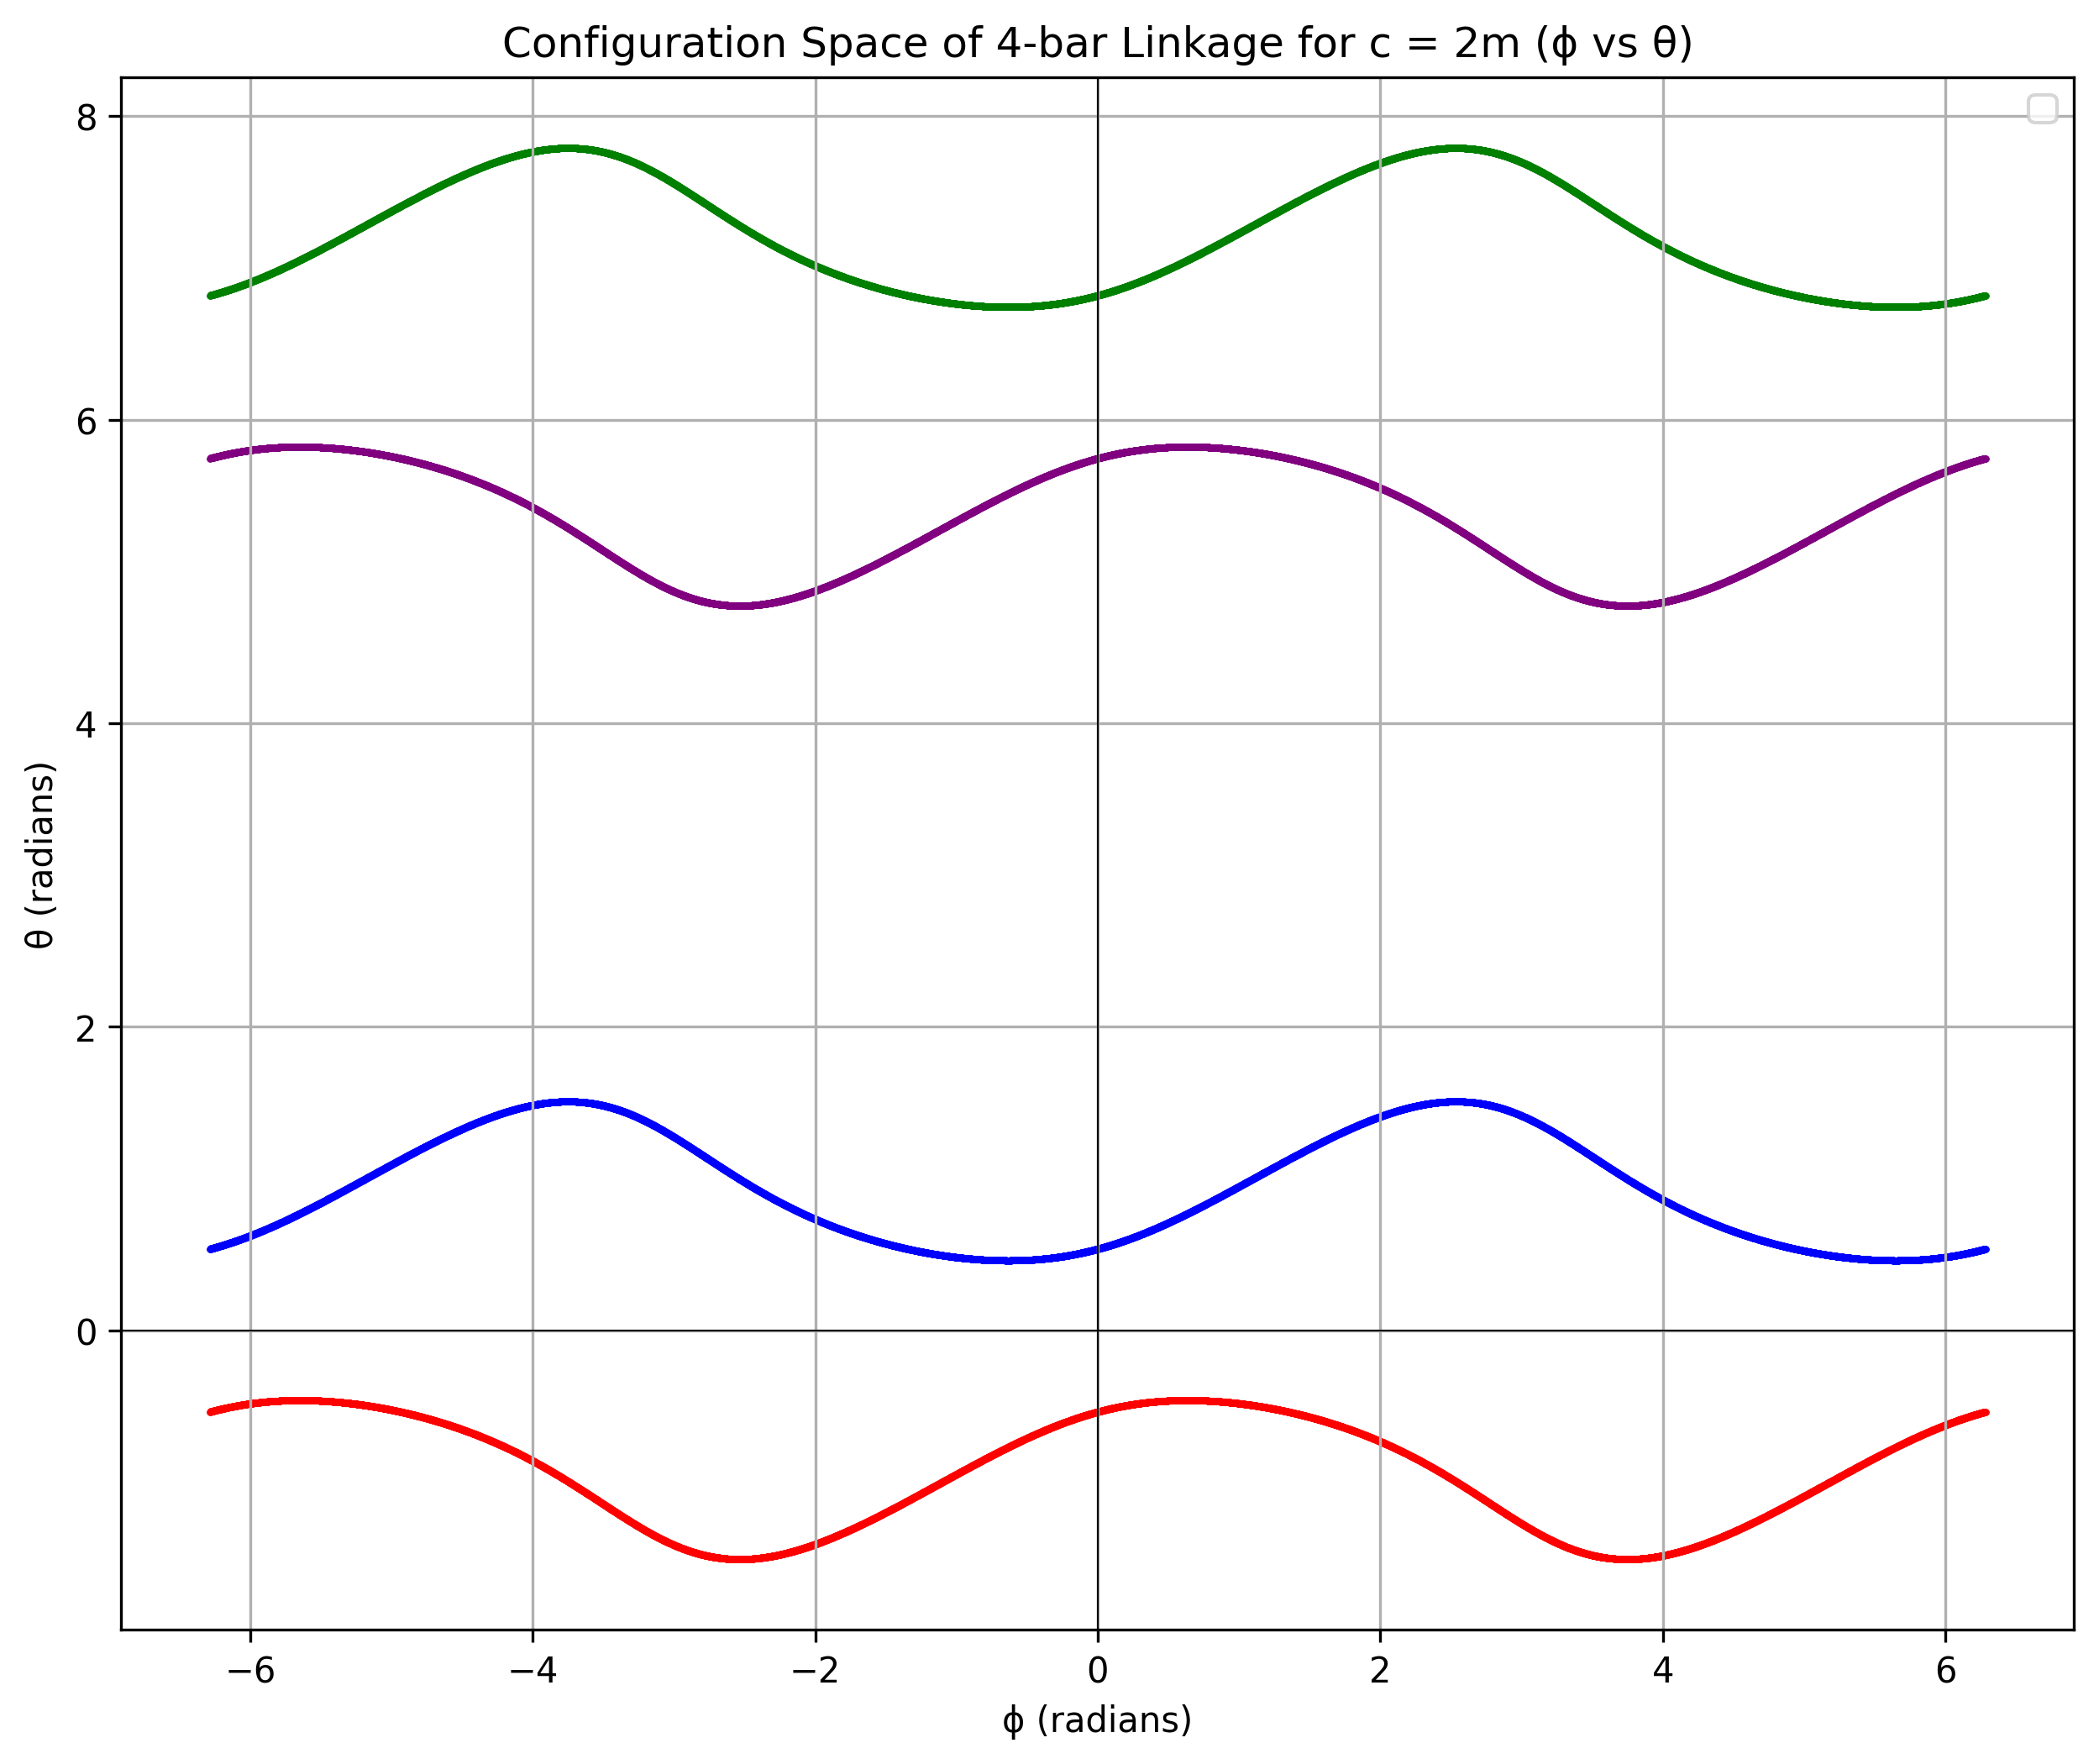
\includegraphics[width=0.8\textwidth]{C:/Users/farha/Desktop/Caltech/2024-2025/EE133a/Hw1/Hw1config_space_c_2m.png}
    \caption{Configuration Space for \( c = 2m \)}
    \label{fig:c_2m}
\end{figure}


\begin{figure}[h!]
    \centering
    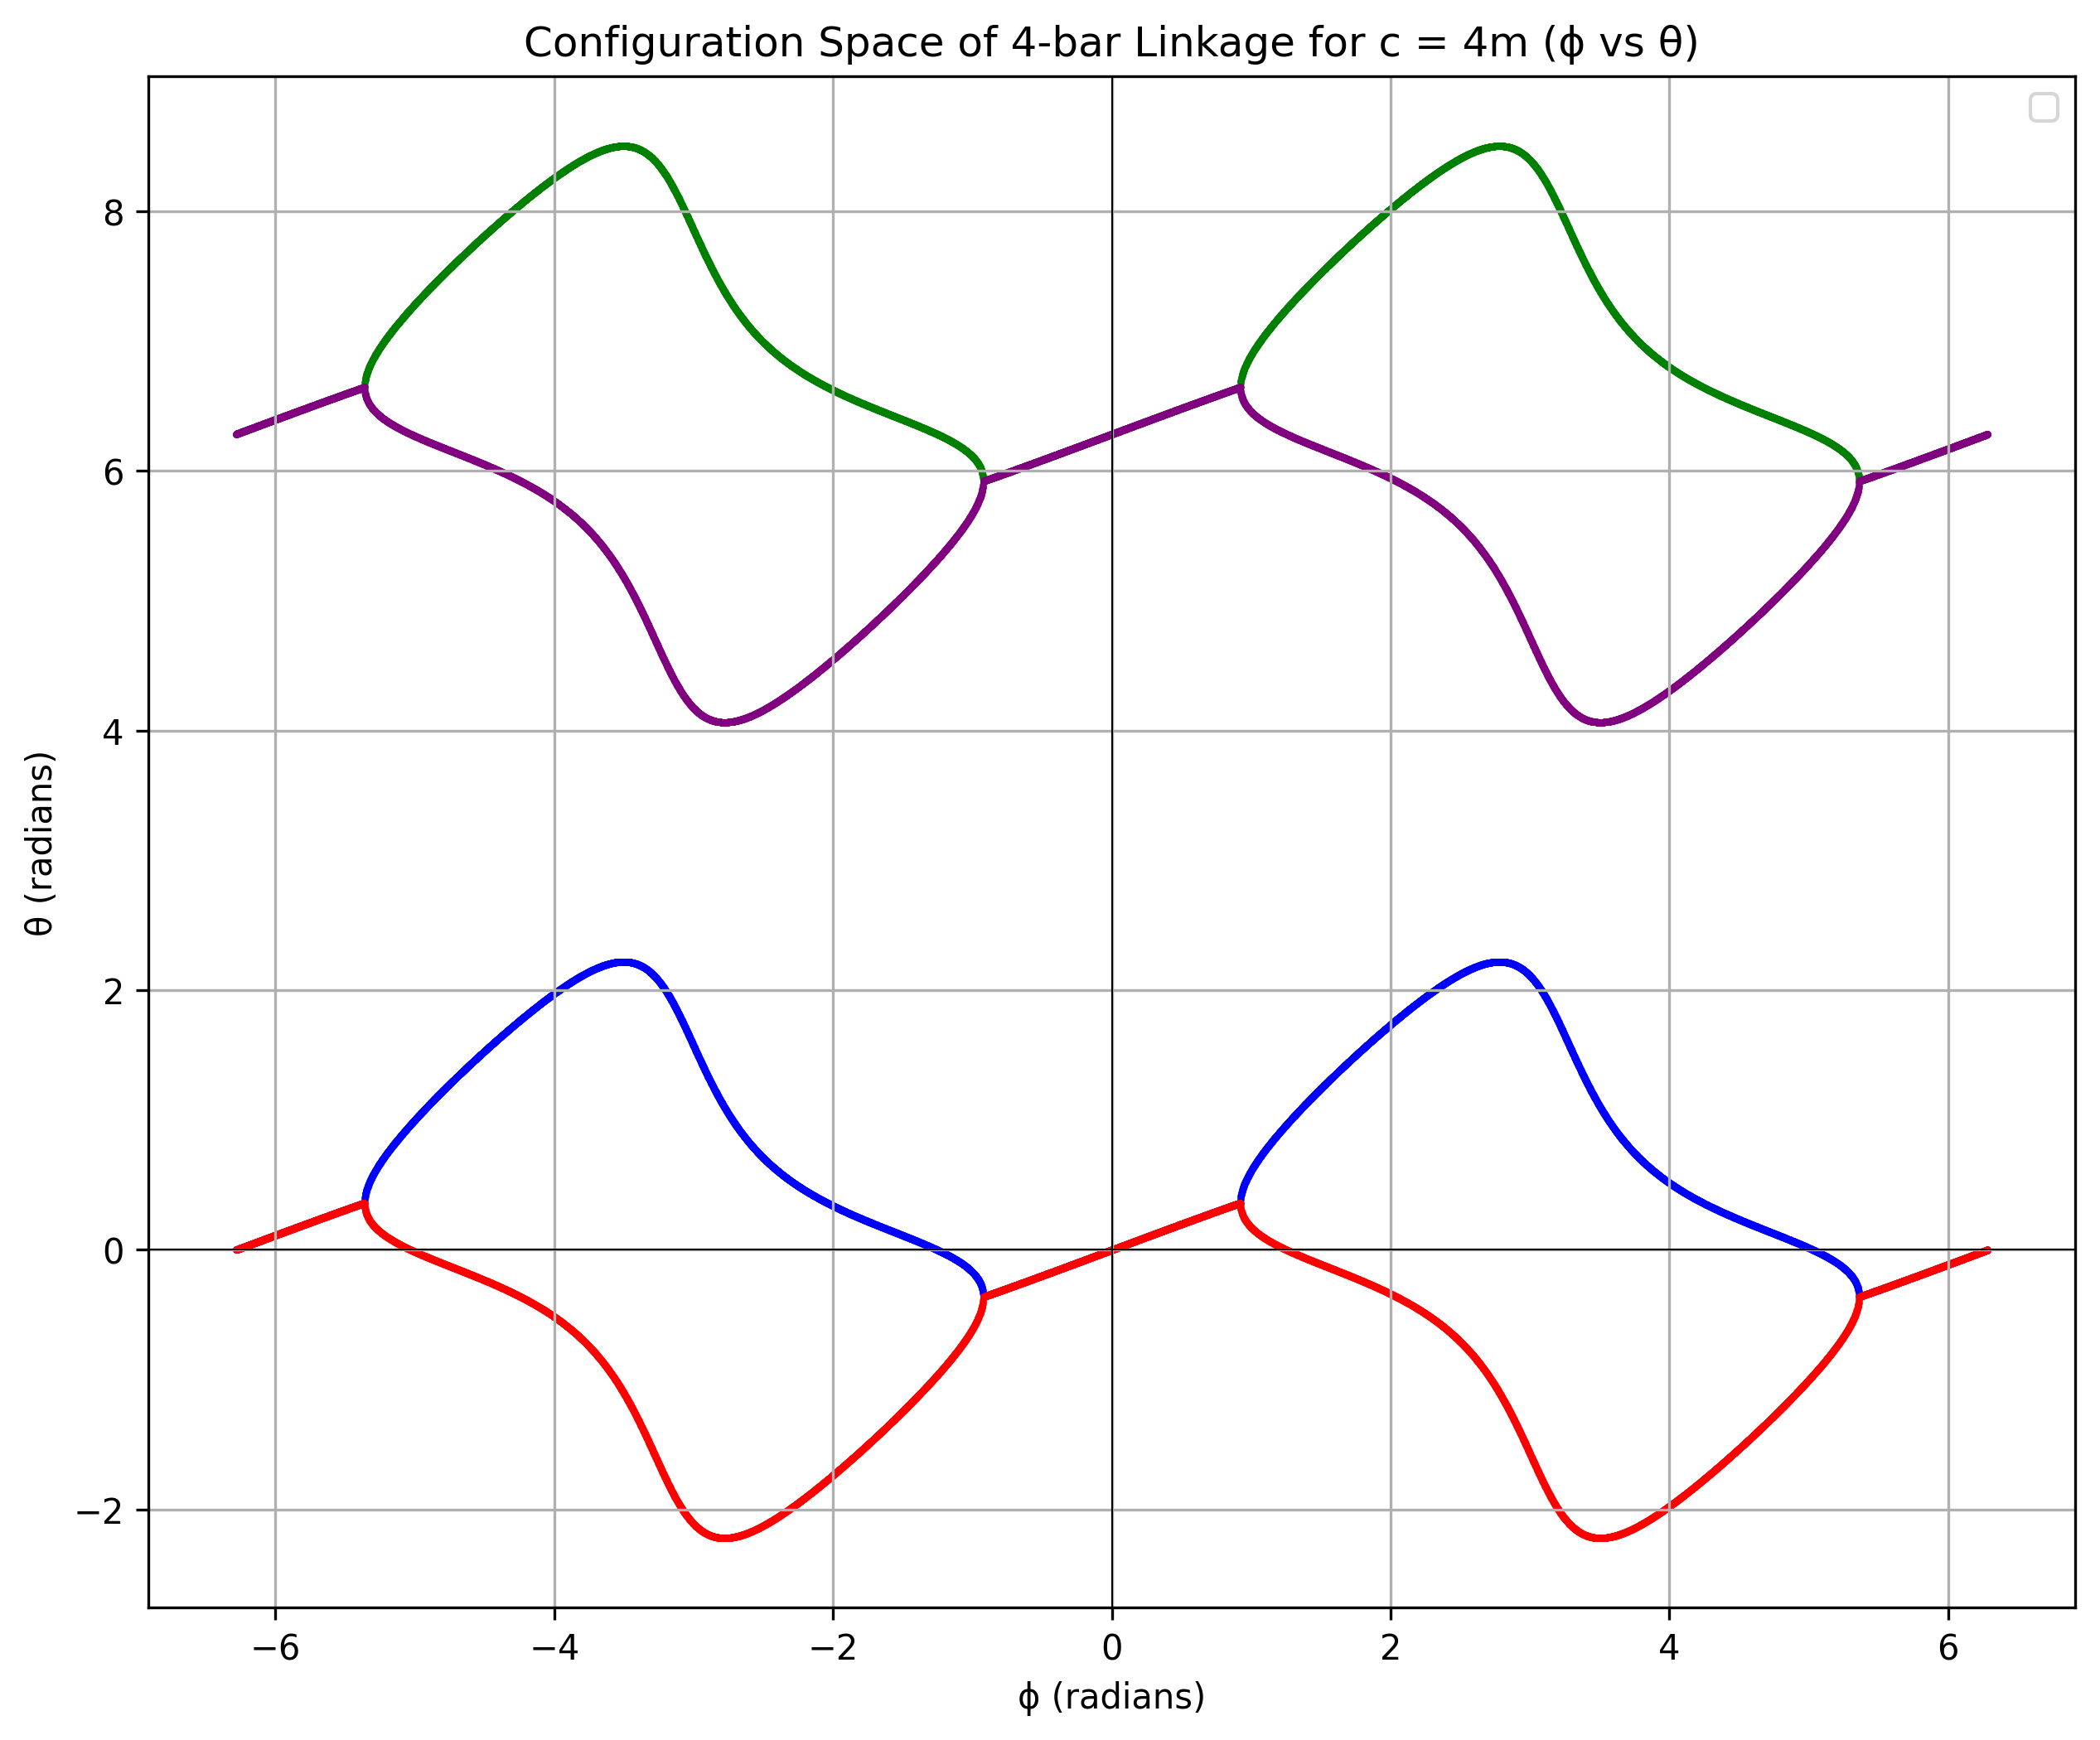
\includegraphics[width=0.8\textwidth]{C:/Users/farha/Desktop/Caltech/2024-2025/EE133a/Hw1/Hw1config_space_c_4m.png}
    \caption{Configuration Space for \( c = 4m \)}
    \label{fig:c_4m}
\end{figure}


\begin{figure}[h!]
    \centering
    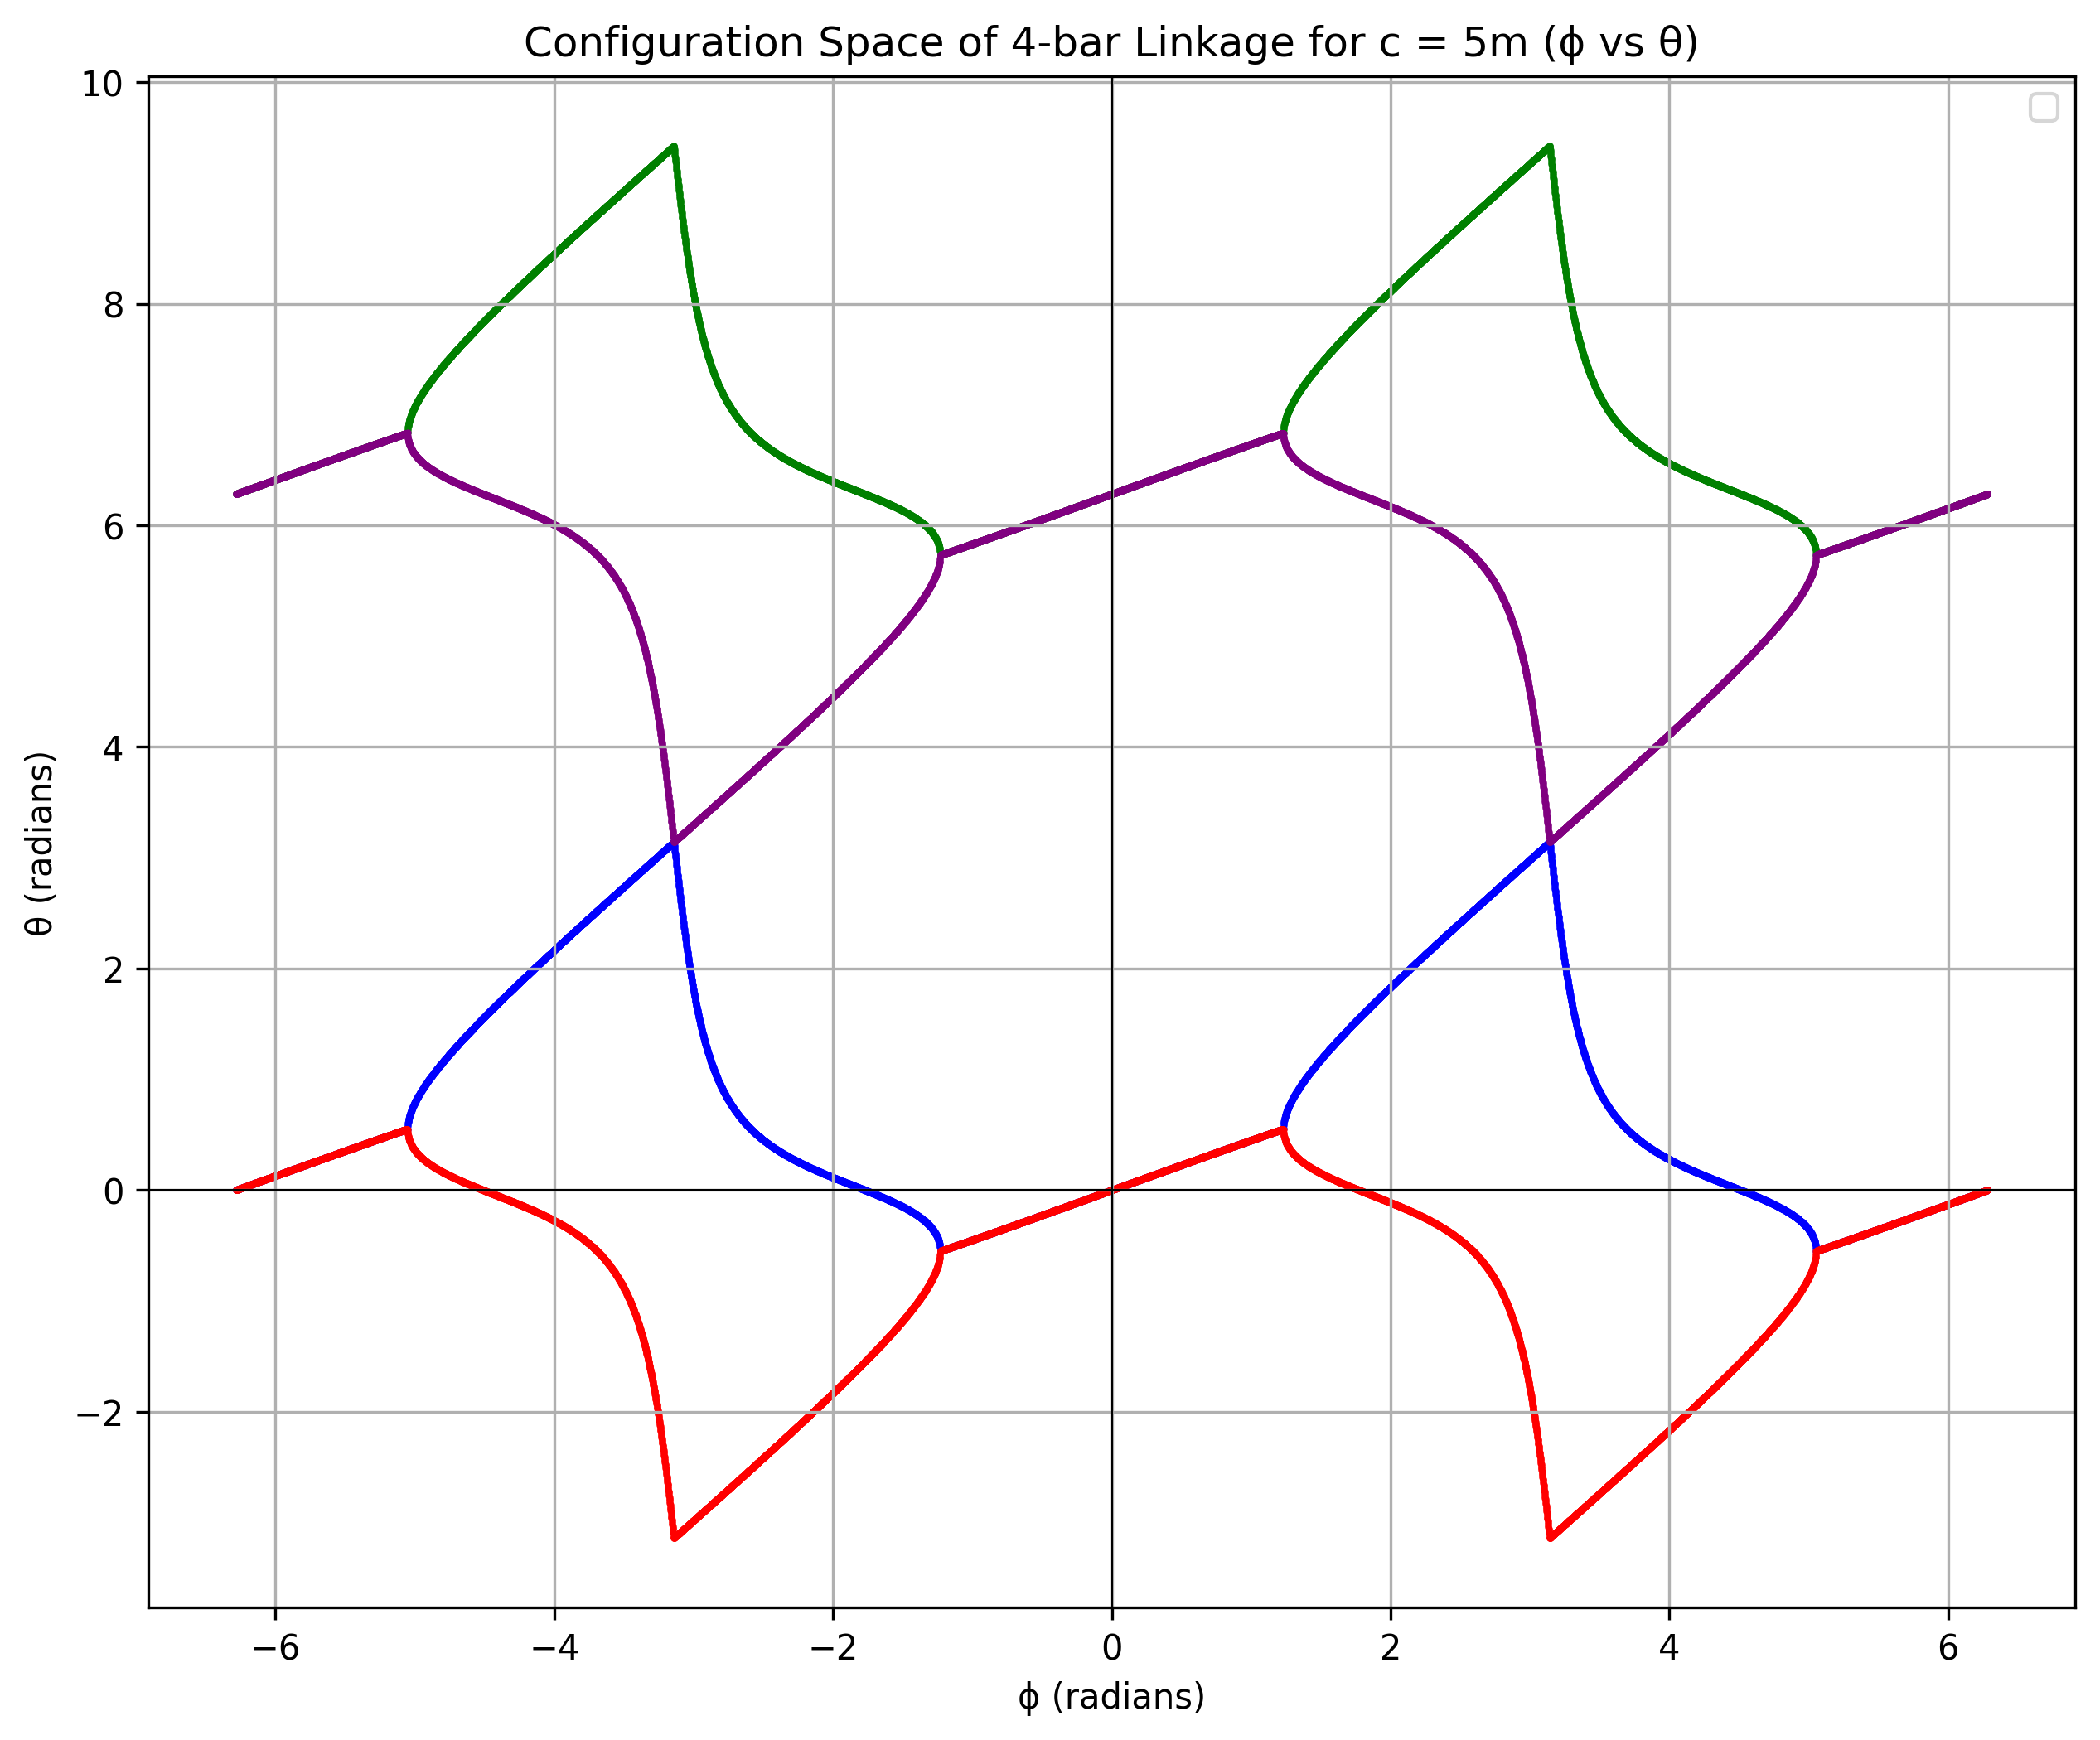
\includegraphics[width=0.8\textwidth]{C:/Users/farha/Desktop/Caltech/2024-2025/EE133a/Hw1/Hw1config_space_c_5m.png}
    \caption{Configuration Space for \( c = 5m \)}
    \label{fig:c_5m}
\end{figure}

\clearpage

\subsection*{Code (pyhton) Used:}

\begin{lstlisting}[language=Python]
    import numpy as np
    import matplotlib.pyplot as plt
    
    a = 4
    b = 5
    d = 6
    
    save_path = r"C:\\Users\\farha\\Desktop\\Caltech\\2024\\EE133a\\Hw1"
    
    def calculate_theta(phi, c):
        XB = d + c * np.cos(phi)
        YB = c * np.sin(phi)
        r = np.sqrt(XB**2 + YB**2)
        cos_beta = (a**2 + r**2 - b**2) / (2 * a * r)
        beta = np.arccos(np.clip(cos_beta, -1, 1))
        gamma = np.arctan2(YB, XB)
        theta_1 = gamma + beta
        theta_2 = gamma - beta
        theta_3 = theta_1 + 2 * np.pi
        theta_4 = theta_2 + 2 * np.pi
        
        return theta_1, theta_2, theta_3, theta_4
    
    phi_values = np.linspace(-2*np.pi, 2*np.pi, 10000)
    c_values = [2, 4, 5]
    
    for c in c_values:
        theta_1_values = []
        theta_2_values = []
        theta_3_values = []
        theta_4_values = []
        
        for phi in phi_values:
            theta_1, theta_2, theta_3, theta_4 = calculate_theta(phi, c)
            theta_1_values.append(theta_1)
            theta_2_values.append(theta_2)
            theta_3_values.append(theta_3)
            theta_4_values.append(theta_4)
        
        plt.figure(figsize=(10, 8))
        plt.scatter(phi_values, theta_1_values, label=f'', color='blue', s=1, marker='o')
        plt.scatter(phi_values, theta_2_values, label=f'', color='red', s=1, marker='o')
        plt.scatter(phi_values, theta_3_values, label=f'', color='green', s=1, marker='o')
        plt.scatter(phi_values, theta_4_values, label=f'', color='purple', s=1, marker='o')
    
        plt.xlabel('ϕ (radians)')
        plt.ylabel('θ (radians)')
        plt.title(f'Configuration Space of 4-bar Linkage for c = {c}m (ϕ vs θ)')
        plt.axhline(0, color='black', linewidth=0.5)
        plt.axvline(0, color='black', linewidth=0.5)
        plt.legend()
        plt.grid(True)
    
        plt.savefig(f"{save_path}config_space_c_{c}m.png", dpi=300, bbox_inches='tight')
    
    plt.show()
    \end{lstlisting}

\clearpage  % Forces the figure to appear before the next section


\section{problem 6}
\subsection*{Deriving Equations:}

Given that:
\[
l_1 = 5 \, \text{m}, \quad l_2 = 1 \, \text{m}, \quad l_3 = 2 \, \text{m}
\]

The angles for the joints are denoted by \( \theta_1 \), \( \theta_2 \), and \( \theta_3 \). We aim to find the possible \( (x, y) \)-coordinates for the end-effector \( P \) by calculating the position for each case where the angles have different constraints.

\subsection*{Position of End-Effector \( P \)}

We can find \( P \) by summing up the positions of the links as follows:

\subsection*{Coordinates for Link 1}
\[
X_1 = l_1 \cos(\theta_1), \quad Y_1 = l_1 \sin(\theta_1)
\]

\subsection*{Coordinates for Link 2}
For the second link:
\[
X_2 = X_1 + l_2 \cos(\theta_1 + \theta_2), \quad Y_2 = Y_1 + l_2 \sin(\theta_1 + \theta_2)
\]

\subsection*{Coordinates for Link 3 (End-Effector)}
For the third link (end-effector point \( P \)):
\[
X_3 = X_2 + l_3 \cos(\theta_1 + \theta_2 + \theta_3), \quad Y_3 = Y_2 + l_3 \sin(\theta_1 + \theta_2 + \theta_3)
\]
Substituting for \( X_2 \) and \( Y_2 \), we can express the position of the end-effector directly in terms of \( \theta_1 \), \( \theta_2 \), and \( \theta_3 \):

\[
X_3 = l_1 \cos(\theta_1) + l_2 \cos(\theta_1 + \theta_2) + l_3 \cos(\theta_1 + \theta_2 + \theta_3)
\]
\[
Y_3 = l_1 \sin(\theta_1) + l_2 \sin(\theta_1 + \theta_2) + l_3 \sin(\theta_1 + \theta_2 + \theta_3)
\]

\subsection*{Workspace Calculation}

Now its possible to calculate the workspace for the three cases (done numericaaly)

\subsection*{Plotting the Workspaces}

Below are the workspaces for each of the three cases:

\begin{figure}[h!]
    \centering
    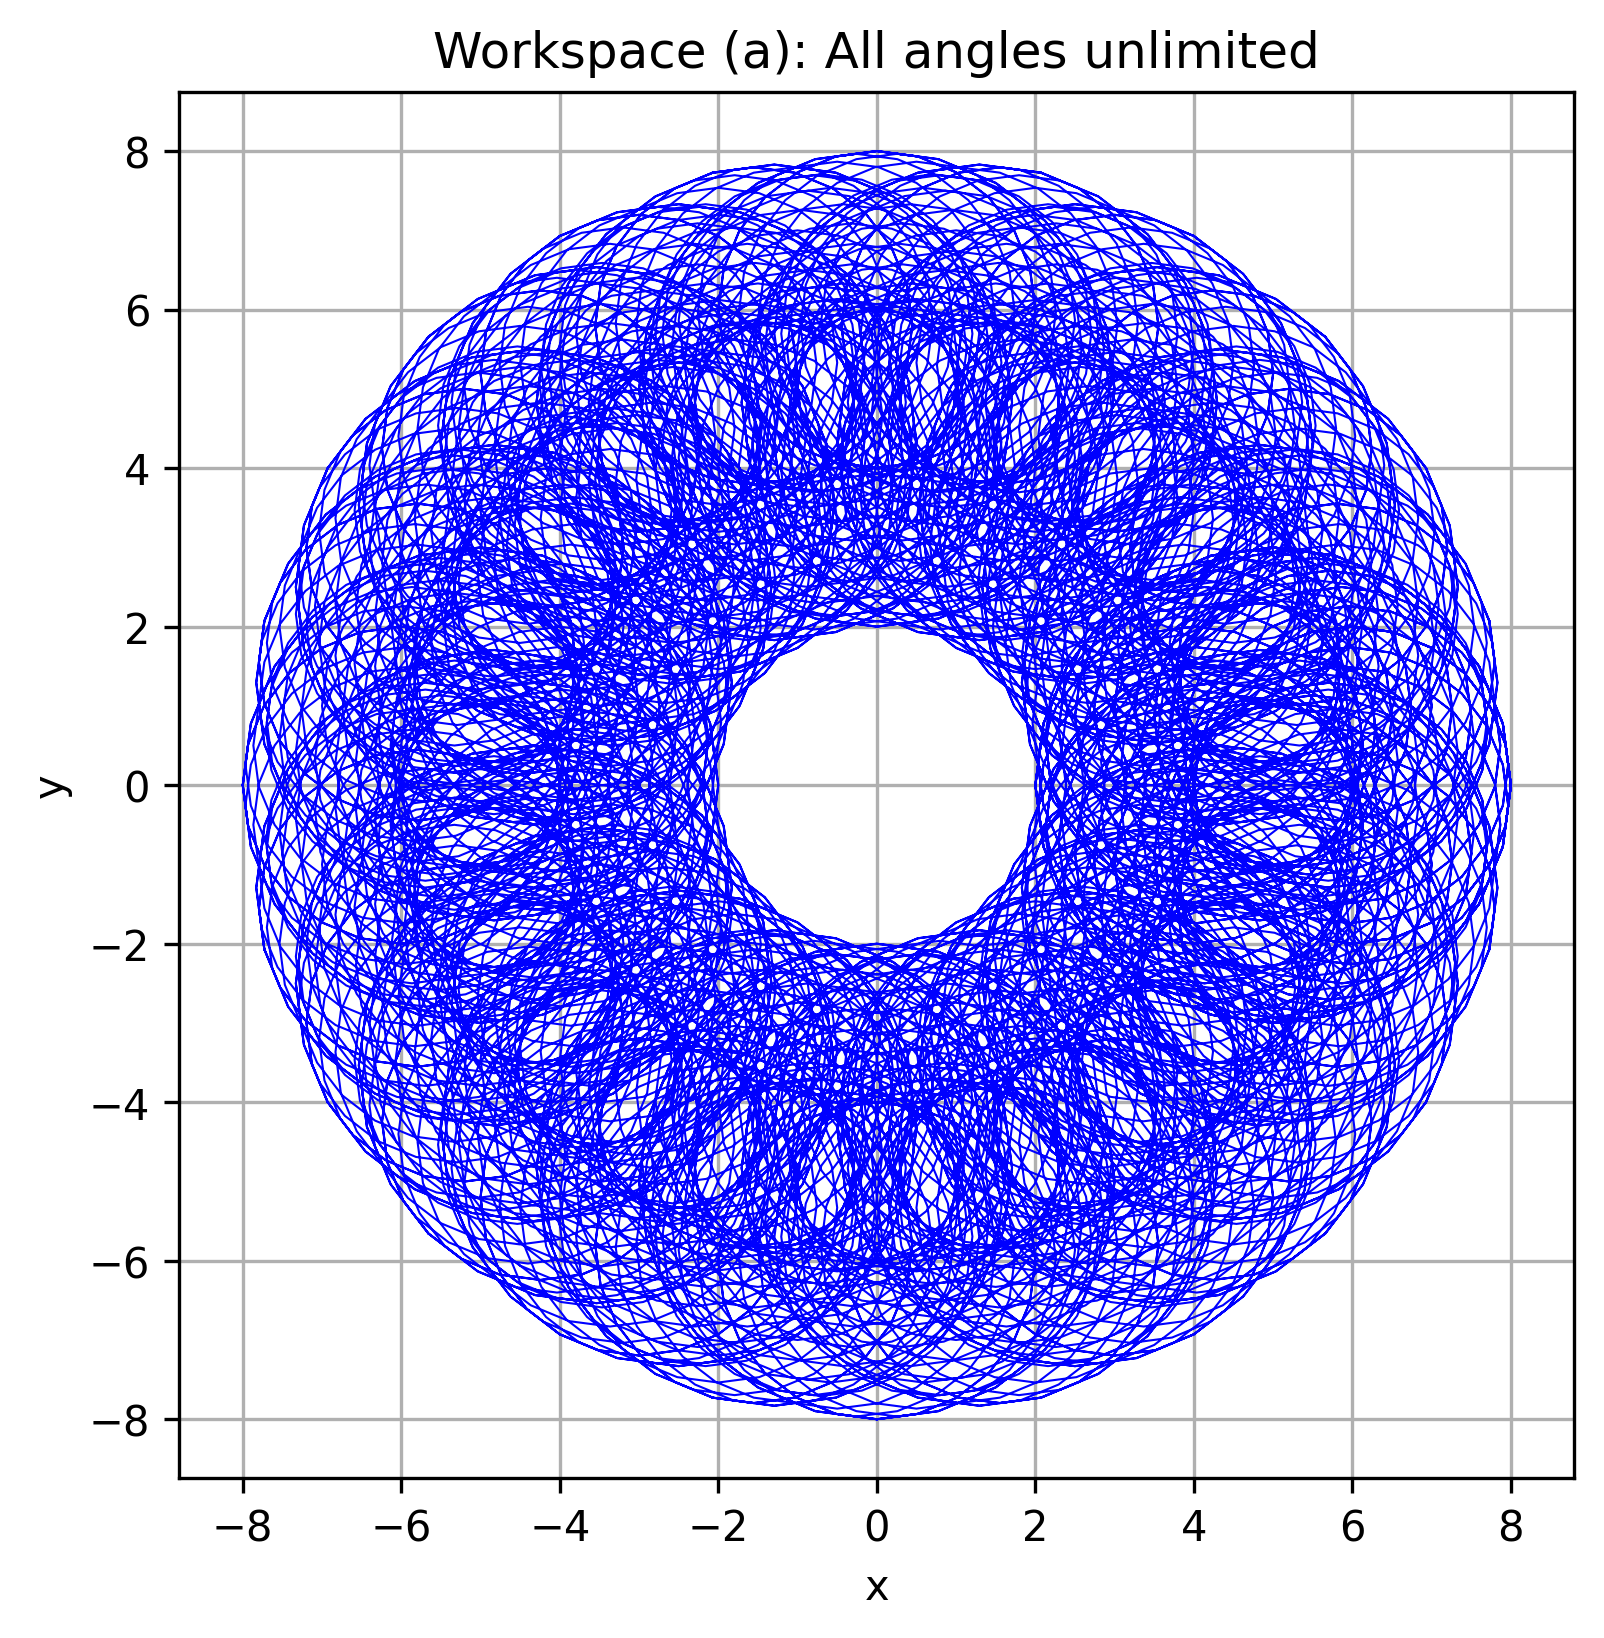
\includegraphics[width=0.8\textwidth]{workspace_case_a.png}
    \caption{Workspace (a): All angles unlimited}
    \label{fig:workspace_case_a}
\end{figure}

\begin{figure}[h!]
    \centering
    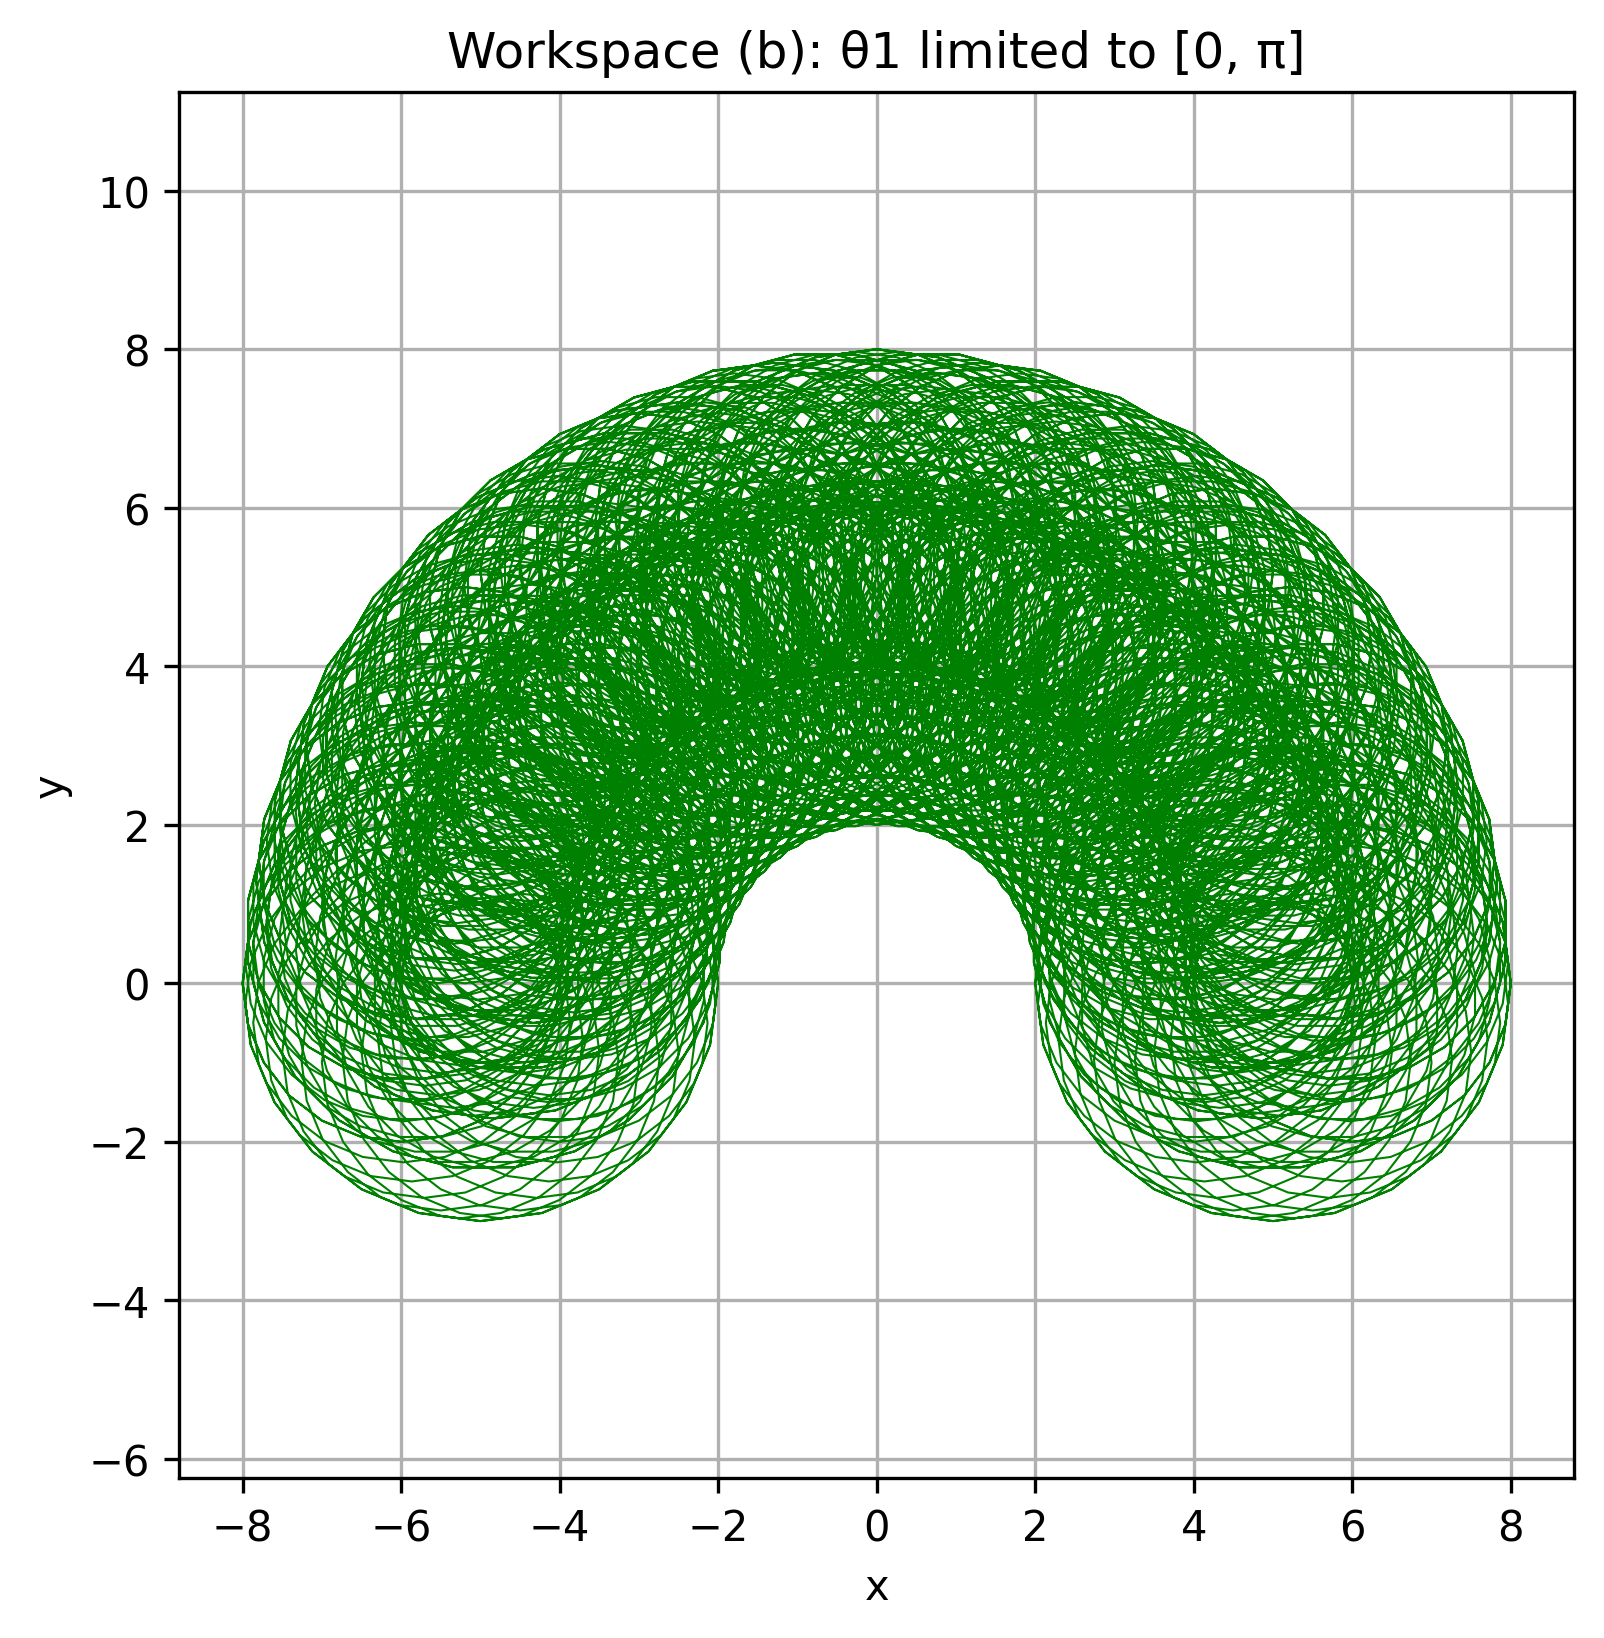
\includegraphics[width=0.8\textwidth]{workspace_case_b.png}
    \caption{Workspace (b): \( \theta_1 \) limited to \( [0, \pi] \)}
    \label{fig:workspace_case_b}
\end{figure}

\begin{figure}[h!]
    \centering
    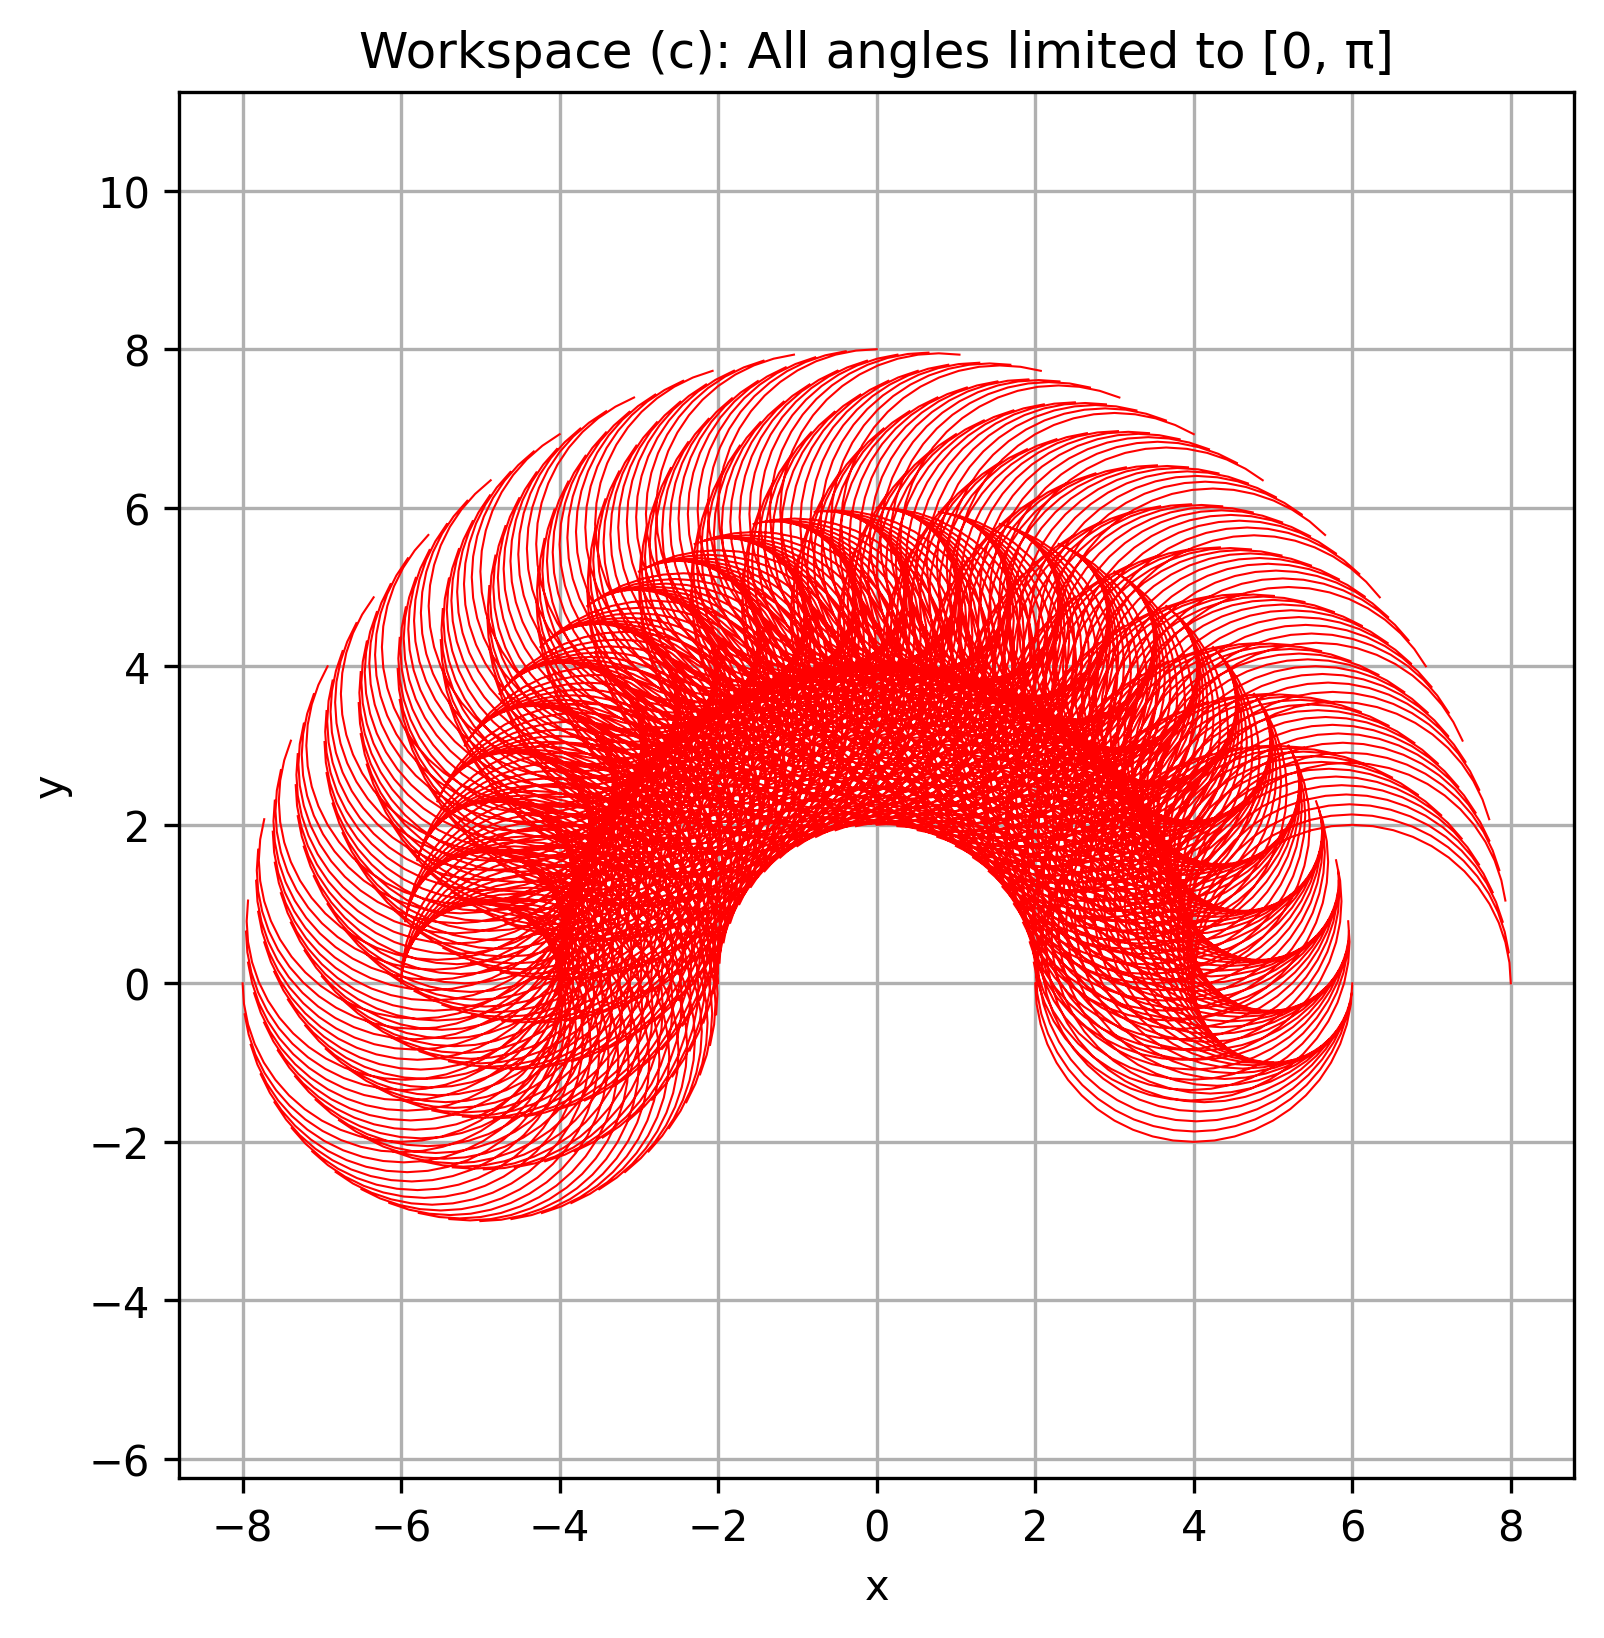
\includegraphics[width=0.8\textwidth]{workspace_case_c.png}
    \caption{Workspace (c): All angles limited to \( [0, \pi] \)}
    \label{fig:workspace_case_c}
\end{figure}

\clearpage
\subsection*{Code (pyhton) Used:}

\begin{lstlisting}[language=Python]
    import numpy as np
    import matplotlib.pyplot as plt
    
    l1 = 5
    l2 = 1
    l3 = 2
    def calculate_workspace(theta1_range, theta2_range, theta3_range, num_points=25):
        theta1_values = np.linspace(theta1_range[0], theta1_range[1], num_points)
        theta2_values = np.linspace(theta2_range[0], theta2_range[1], num_points)
        theta3_values = np.linspace(theta3_range[0], theta3_range[1], num_points)
        
        X = []
        Y = []
        for theta1 in theta1_values:
            for theta2 in theta2_values:
                for theta3 in theta3_values:
                    x = l1 * np.cos(theta1) + l2 * np.cos(theta1 + theta2) + l3 * np.cos(theta1 + theta2 + theta3)
                    y = l1 * np.sin(theta1) + l2 * np.sin(theta1 + theta2) + l3 * np.sin(theta1 + theta2 + theta3)                
                    if len(X) > 0 and np.sqrt((x - X[-1])**2 + (y - Y[-1])**2) > 1.0:
                        X.append(None)  
                        Y.append(None)  
                    
                    X.append(x)
                    Y.append(y)
        
        return np.array(X), np.array(Y)
    
    def plot_and_save_workspace(X, Y, title, filename, color='blue'):
        plt.figure(figsize=(6, 6))
        plt.plot(X, Y, color=color, linewidth=0.5)
        plt.title(title)
        plt.xlabel('x')
        plt.ylabel('y')
        plt.axis('equal')
        plt.grid(True)
        plt.savefig(f'{filename}.png', dpi=300, bbox_inches='tight')
        plt.show()
    
    theta1_range_a = [0, 2*np.pi]
    theta2_range_a = [0, 2*np.pi]
    theta3_range_a = [0, 2*np.pi]
    X_a, Y_a = calculate_workspace(theta1_range_a, theta2_range_a, theta3_range_a)
    
    theta1_range_b = [0, np.pi]
    theta2_range_b = [0, 2*np.pi]
    theta3_range_b = [0, 2*np.pi]
    X_b, Y_b = calculate_workspace(theta1_range_b, theta2_range_b, theta3_range_b)
    
    theta1_range_c = [0, np.pi]
    theta2_range_c = [0, np.pi]
    theta3_range_c = [0, np.pi]
    X_c, Y_c = calculate_workspace(theta1_range_c, theta2_range_c, theta3_range_c)
    
    plot_and_save_workspace(X_a, Y_a, 'Workspace (a): All angles unlimited', 'workspace_case_a', color='blue')
    plot_and_save_workspace(X_b, Y_b, 'Workspace (b): θ1 limited to [0, π]', 'workspace_case_b', color='green')
    plot_and_save_workspace(X_c, Y_c, 'Workspace (c): All angles limited to [0, π]', 'workspace_case_c', color='red')
    
    \end{lstlisting}
\newpage
\section{Problem 7}
\item Time Spent was around 5 hours.

\end{document}